%%%%%%%%%%%%%%%%%%%%%%%%%%
%%% author : Yamada. T %%%
%%% made for TH series %%%
%%%%%%%%%%%%%%%%%%%%%%%%%%

\documentclass[b5paper,10pt,fleqn] {ltjsarticle}

\usepackage[margin=10truemm]{geometry}

\usepackage{pict2e, graphicx}
\usepackage{tikz}
\usetikzlibrary{intersections,calc,arrows.meta}

\usepackage{amsmath, amssymb, amsthm}
\usepackage{ascmac}
\usepackage{comment}
\usepackage{empheq}
\usepackage[shortlabels,inline]{enumitem}
\usepackage{fancybox}
\usepackage{fancyhdr}
\usepackage{here}
\usepackage{lastpage}
\usepackage{listings, jvlisting}
\usepackage{fixdif}

\usepackage{stmaryrd}
\usepackage[listings]{tcolorbox}
%\usepackage{ascolorbox}
\usepackage{titlesec}
\usepackage{ulem}
\usepackage{url}
\usepackage{verbatim}
\usepackage{wrapfig}
\usepackage{xcolor}
\usepackage{luatexja-ruby}
\usepackage{varwidth}
\usepackage[version=3]{mhchem}
\usepackage{wrapfig}


\usepackage{physics2}
	\usephysicsmodule{ab}
	\usephysicsmodule{ab.braket}
	\usephysicsmodule{ab.legacy}
	%\usephysicsmodule{braket}
	\usephysicsmodule{diagmat}
	\usephysicsmodule{xmat}
	\usephysicsmodule{nabla.legacy}
	\usephysicsmodule{qtext.legacy}

\usepackage[ISO]{diffcoeff}
\difdef { f, s } { D }
{ op-symbol = \mathrm{D} }


\newcommand{\mctext}[1]{\mbox{\textcircled{\scriptsize{#1}}}}
\newcommand{\ctext}[1]{\textcircled{\scriptsize{#1}}}
\newcommand{\ds}{\displaystyle}
\newcommand{\comb}[2]{{}_{#1}\mathrm{C}_{#2}}
\newcommand{\hs}{\hspace}
\newcommand{\vs}{\vspace}
\newcommand{\emphvs}{\vspace{1em}\notag\\}
\newcommand{\ora}{\overrightarrow}
\newcommand{\ol}{\overline}
\newcommand{\oramr}[1]{\overrightarrow{\mathrm{#1}}}
\newcommand{\tri}{\triangle}
\newcommand{\mr}{\mathrm}
\newcommand{\mb}{\mathbb}
\newcommand{\mrvec}[1]{\overrightarrow{\mathrm{#1}}}
\newcommand{\itvec}{\overrightarrow}
\newcommand{\bs}{\boldsymbol}
\newcommand{\ra}{\rightarrow}
\newcommand{\Ra}{\Rightarrow}
\newcommand{\lra}{\longrightarrow}
\newcommand{\Lra}{\Longrightarrow}
\newcommand{\la}{\leftarrow}
\newcommand{\La}{\Leftarrow}
\newcommand{\lla}{\longleftarrow}
\newcommand{\Lla}{\Longleftarrow}
\newcommand{\lr}{\leftrightarrow}
\newcommand{\llr}{\longleftrightarrow}
\newcommand{\Llr}{\Longleftrightarrow}
\renewcommand{\deg}{{}^\circ}
\newcommand{\phbox}{\fbox{\phantom{1\hspace{2em}}}}
\newcommand{\boxnum}[1]{\fbox{\phantom{\hspace{1em}}({#1})\phantom{\hspace{1em}}}}
\newcommand{\boxkana}[1]{\fbox{\phantom{\hspace{1em}}{#1}\phantom{\hspace{1em}}}}
\newcommand{\boxkm}[2]{\fbox{\, {#1}\phantom{\hspace{0.2em}} \,  {#2}}}
\newcommand{\hzw}{\hspace{1\zw}}

\renewcommand{\baselinestretch}{1.25}
\parindent=1\zw

%入82
\begin{document}
\noindent
\fbox{NewTH1-11} [同志社大]

\begin{wrapfigure}{r}{5cm}
  \centering
  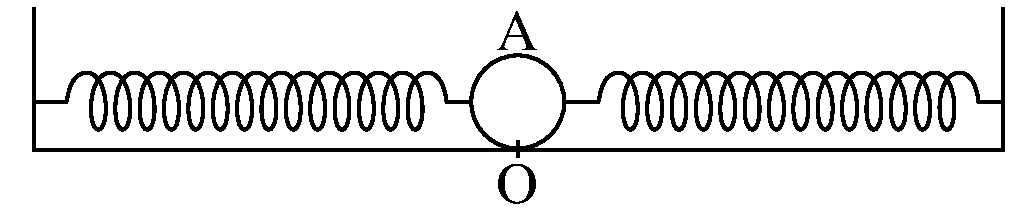
\includegraphics[width=5cm]{fig/fig_1_11_1.pdf}
  
  図1
  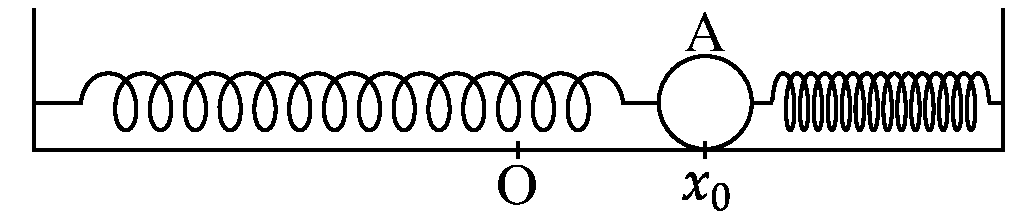
\includegraphics[width=5cm]{fig/fig_1_11_2.pdf}

  図2
\end{wrapfigure}


次の文中の空欄\boxkana{ア}〜\boxkana{サ}に当てはまる式を記せ.
また,解答図(A)には適切なグラフの概形を描け.
ただし,重力加速度の大きさを$g$とする.

図1に示すように,質量$m$の小球Aがばね定数$k$の2本のばねの間につながれて,水平なあらい床の上に置かれて静止している.
2本のばねは,ともに他端が固定され,自然の長さの状態で直線上にある.
このときのAの位置を原点Oとして,水平方向右向きに$x$軸をとる.
床とAの間の静止摩擦係数を$\mu$とし,動摩擦係数を$\mu' \ (< \mu)$とする.

図2のように,Aを位置$x_0$まで右向きに変位させて静かに手をはなすと,Aは左向きに動き始め,$x < 0$のある点$\mr{P}_1$で速度が0となり,その後運動の向きを右向きに反転し,$x > 0$の領域に入る.Aは,$x > 0$のある点$\mr{P}_2$で速度が0となり,その後運動の向きを左向きに反転する.Aの速度が0となる点を時間経過の順に表すと$\mr{P}_1$,$\mr{P}_2$,$\mr{P}_3$,$\mr{P}_4$となり,Aは$\mr{P}_4$で速度が0となった後,その位置で動かなくなった.


\begin{wrapfigure}{r}{6cm}
  \hspace{0cm}(A)

  \centering
  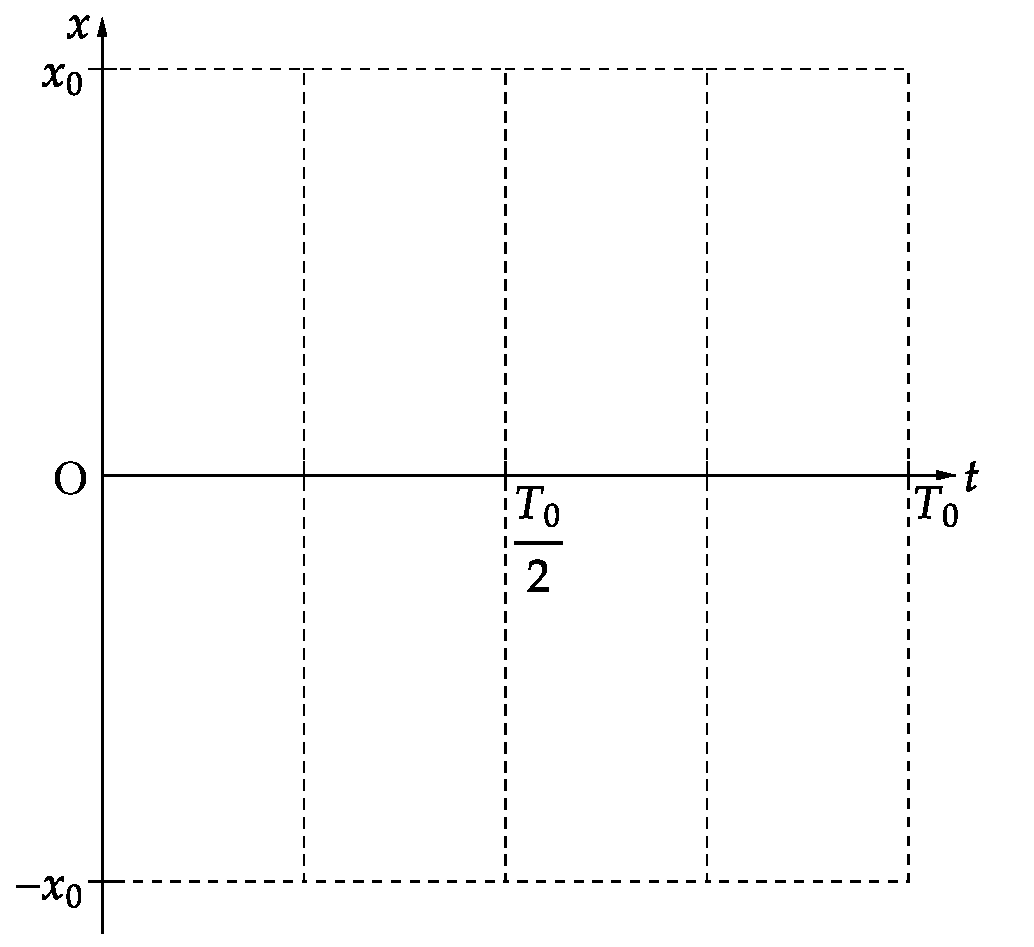
\includegraphics[width=6cm]{fig/fig_1_11_3.pdf}
\end{wrapfigure}
Aが位置$x$を左向きに運動しているときにAに作用する合力の$x$成分は\boxkana{ア}であり,Aの速度が0となる点に達するまでのAの左向きの運動は$x$軸上の位置$x = \text{\boxkana{イ}}$を振動の中心とする単振動の半周期分の運動である.
同様に,Aの右向きの運動は$x$軸上の位置$x = \text{\boxkana{ウ}}$を中心とする単振動の半周期分の運動である.
Aが最初に原点Oを左向きに通過するときの速さは\boxkana{エ}であり,
最初に運動の向きが反転する$\mr{P}_1$の位置は$x = \text{\boxkana{オ}}$である.
運動の向きが反転するたびに原点から速度が0となる点までの距離は\boxkana{カ}だけ小さくなる.
Aが運動を始めてから$\mr{P}_4$で静止するまでに要する時間は\boxkana{キ}であり,その間に摩擦力がAに対してした仕事の大きさは\boxkana{ク}である.
速度が0となる点でAが静止したまま動かなくなる条件は,
原点からその点までの距離が\boxkana{ケ}より小さくなることであり,
$\mr{P}_4$で初めてこれが満たされたことになる.
$T_0$を床とAの間に摩擦がない場合のAの単振動の周期として,解答図(A)にAが動き始めてから時間$T_0$だけ経過するまでの,
Aの位置の時間変化を表すグラフの概略を実線で,
また,各半周期分の振動の中心位置の時間変化を表すグラフの概略を破線で描け.
グラフの横軸は時間,縦軸は$x$方向の位置である.

Aの最初の位置を$x_0$から$x_1\ ( > x_0)$に変更して,$n$回目に速度が0となる点$\mr{P}_n$でAが静止したまま動かなくなるようにしたい.
このとき$\mr{P}_{n-1}$でAが止まったままとはならずに動くことから$x_1 > \text{\boxkana{コ}}$である必要がある.
これに加えて,$\mr{P}_n$でAが止まったままとなることから,$x_1 \leqq \text{\boxkana{サ}}$である必要がある.
ばねが短いとこれらの条件は満たされないので,ばねが十分に長いことも必要である.
\end{document}